% !TeX root = Main_file.tex
\documentclass[12pt,fleqn]{article}
\usepackage{a4}
\usepackage{graphicx}
\usepackage{psfrag}
\usepackage{amsmath}                     % \boldsymbol{#1}
\usepackage{amssymb}
%\usepackage{hangcaption}
%\usepackage{Styles/pstricks}
%\usepackage{Styles/pst-node}
\usepackage{Styles/fancyheadings}
\usepackage{tocloft}
\usepackage[euler]{textgreek}
%\usepackage{mathtools}
%\usepackage{unicode-math}
%\setmathfont{XITS Math}
%\newcommand*{\matr}[1]{\mathbfit{#1}}
%\newcommand*{\tran}{^\mkern-1.5mu\mathsf{T}}}
%\newcommand*{\conj}[1]{\overline{#1}}
%\newcommand*{\hermconj}{^{mathsf{H}}}
\usepackage{MnSymbol}
%\usepackage{breqn}
%-----Tex width---------------------------------
\textwidth 16cm

%-----Line spacing-------------------------------
\renewcommand{\baselinestretch}{1.5}     % 1,1-zeilig

%---------Add dots in TOC-----------------------
\renewcommand{\cftsecleader}{\cftdotfill{\cftdotsep}}

%------Paragraph indention-------------------------------
\setlength{\parskip}{1.5ex plus0.5ex minus0.5ex}

%-----Prevent indent----------------------
\setlength{\parindent}{0em}

%-----Richtiger Abstand fur Einheiten-------------
\def\Unit{\hspace{0.25em}}

%-----Definition of the header--------------------
\pagestyle{fancyplain}
\renewcommand{\sectionmark}[1]{\markboth{Chapter~\thesection.~#1}{#1}}
\renewcommand{\subsectionmark}[1]{\markright{\thesubsection\ #1}}
\rhead[\fancyplain{}{\leftmark}]%
{\fancyplain{\thepage}{\thepage}} \cfoot{} \plainheadrulewidth
0.4pt
%% Otherwise: Overfull \vbox-Warning against fancyheadings-pacakage
%%  idea of: nic@minster.york.ac.uk (Nick Cropper)
\makeatletter
\ifcase \@ptsize \relax % 10pt
  \addtolength{\headheight}{1\p@}
\or % 11pt
  \addtolength{\headheight}{2\p@}
\or % 12pt
  \addtolength{\headheight}{3\p@}
\fi \makeatother

%-----Equations / Figures / Tables numbering according to \ sections
\makeatletter
\renewcommand\theequation{\thesection.\arabic{equation}}
\renewcommand\thefigure{\thesection.\arabic{figure}}
\renewcommand\thetable{\thesection.\arabic{table}}
\@addtoreset{equation}{section} \@addtoreset{figure}{section}
\@addtoreset{table}{section} \makeatother

%-----Useful abbreviations----------------------
\newcommand{\mr}{\mathrm}
%%\newcommand{\bs}[1]{\mbox{$\boldsymbol{#1}$}}
\newcommand{\degree}[1]{\mbox{$#1^\circ$}}

%\renewcommand{\figurename}{Bild}

%------Bibliography style-----------------------
\bibliographystyle{IEEEtran}

%-----Aufzaehlunstiefe im Literaturverzeichnis---------------
\setcounter{tocdepth}{3}

\begin{document}
\pagenumbering{Roman}
\begin{titlepage}
  \begin{center}
      \vspace*{-4.0cm}
    \begin{figure}[!h]
\centering

\includegraphics[width=0.3\linewidth]{Figures/JKUAT_logo}
%\caption{}
\label{fig:jomologo}
\end{figure}
   \large{Jomo Kenyatta University of Agriculture and Technology}\\
    \large{College of Engineering and Technology}\\
    \large{School of Mechanical, Materials, and Manufacturing Engineering}\\
   \large{Department of Marine Engineering and Maritime Operations}\\

    ------------------------------------------------------------------------------------------------\\[1.0cm]
    \LARGE{\textbf{Advanced Condition Based Predictive
    		Maintenance of Electric Motors in Ships}}\\[0.6cm]
    	
    \large{\textbf{MR-PRO-22-010}}\\[0.4cm]
    \LARGE{\textbf{Final year Project 
            }}\\[1.5cm]
    %\large{by}\\[0.6cm

    \vspace{0.5cm}
    
            
     \large{\textbf{Kibichii Kieran~(ENM241-0127/2017)
            }}\\[1.0cm]
%     \large{\textbf{Supervisors}}\\
%    \large{Dr.-Ing.~Jackson G. Njiri}\\
%    \large{Prof. George N. Nyakoe}\\
%    \large{\ldots}    \\[0.2cm]\vfill
    \large{\small{\today}}\\
    ------------------------------------------------------------------------------------------------\\[1.5cm]
  \end{center}
\end{titlepage}
%
%\pagenumbering{gobble}% Remove page numbers (and reset to 1)

\addcontentsline{toc}{section}{Declaration}
\section*{Declaration}

We hereby declare that the work contained in this report is original; researched and documented by the undersigned students. It has not been used or presented elsewhere in any form for award of any academic qualification or otherwise. Any material obtained from other parties have been duly acknowledged. We have ensured that no violation of copyright or intellectual property rights have been committed.
\begin{enumerate}

	\item Kibichii Kieran\vspace*{.2cm}\\
	Signature\ldots\ldots\ldots\ldots\ldots\ldots\ldots\ldots\ldots\ldots Date\ldots\ldots\ldots\ldots\ldots\ldots\ldots\ldots\ldots\ldots
\end{enumerate}

\vspace*{.5cm}
Approved by supervisors:
\begin{enumerate}
	\item Dr. Benson Oyunge \vspace*{.2cm}\\
	Signature\ldots\ldots\ldots\ldots\ldots\ldots\ldots\ldots\ldots\ldots Date\ldots\ldots\ldots\ldots\ldots\ldots\ldots\ldots\ldots\ldots

	\item Dr. Gerald J. Odhiambo\vspace*{.2cm}\\
	Signature\ldots\ldots\ldots\ldots\ldots\ldots\ldots\ldots\ldots\ldots Date\ldots\ldots\ldots\ldots\ldots\ldots\ldots\ldots\ldots\ldots
\end{enumerate}



\clearpage
\addcontentsline{toc}{section}{Table of Contents}
\tableofcontents
\clearpage
\addcontentsline{toc}{section}{List of Figures}
{%
\let\oldnumberline\numberline%
\renewcommand{\numberline}{\figurename~\oldnumberline}%
\listoffigures
\clearpage
\addcontentsline{toc}{section}{List of Tables}
\listoftables
\newpage
\clearpage
\addcontentsline{toc}{section}{List of Abbreviations}
\clearpage
\newpage

\newpage
\addcontentsline{toc}{section}{Abstract}

\section*{Abstract}
\label{sec:Abstract}
Maritime shipping is employed to move food, medicines, and far more at the heart of world
trade. For growth and development, economical mechanisms of shipping are followed,
particularly within the developing world. Machinery and equipment breakdown that occur
during marine transportation cause delays, swings in supplies, production, and trigger
infinite downstream effects on entire supply chains.

 In the shipping industry planned and
reactive maintenance that is primarily practiced requires halting of vessel operations for a
number of days despite the fact that no fatigue or machinery and equipment breakdown is
observed. Having seen the importance of motors that are widely utilized in ships auxiliary
machinery, the project focuses on creating failure predictions, additionally determining
remaining useful life (RUL) for motors aboard ships, albeit also quite fascinating is the
role this research plays in the monitoring of equipment on autonomous ships. This is
made possible with developments in information and technology. Massive amounts of
data is collected and can facilitate condition based monitoring (CBM), conduct analysis
on best performance and comprehensively diagnose ship engine room equipment.

Keywords: efficiency, condition monitoring, remaining useful life, autonomous ships, performance. 

 



\clearpage
\pagenumbering{arabic}
  \section{Introduction}
\label{sec:introduction}
\subsection{Background}
\subsubsection{Maintenance}
As the world’s industries push the boundaries of optimization and efficiency, the exponential increase in computational ability and technology The automation of “higher-level” tasks that require human intellect is now possible. This headway brings unmanned autonomous vessels within the maritime industry closer to mass production. The practicality of autonomous vessels can only be achieved with constant awareness of the performance and operating state of machinery in the engine room. Observations of industry practices display that industry experience in reliability is heavily based on trial-and-error test procedures. Most of the reliability research in industry still focuses on two distinct periods of the product life. The warranty period, where most of the failures are due to product malfunctions or quality related problems, and, wear-out period, where the failures are due excessive wear and use \cite{thomas_warranty_1999}. Using sensors and logging software the condition of equipment is assessed as frequently as needed, enabling efficient analysis of data that facilitates planning of predictive maintenance on-board vessels. The electric motor is the most used device for conversion of energy from electric energy to mechanical energy and is used for electric propulsion, powering thrusters for station keeping, and different on-board equipment on hundreds of ships. Typically, 80-90 percent of the load installations will be electric motors\cite{han_motor_2019}.Smart organizations know they can no longer afford to see maintenance as just an expense. Rather, maintenance must be integrated within the business cycle in order to guarantee predictability, growth and increase the overall quality of operations. Moving from a regime of scheduled rule-based maintenance via on-condition maintenance and ultimately to a data-driven risk-based regime can lead to more accurate and timely maintenance tasks. This smarter view of maintenance allows for achieving many practical advantages leading to lower costs and increased safety and availability of ship systems\cite{han_motor_2019}. 
 Making failure predictions and determination of remaining useful life (RUL), realizes significant benefits not limited to: work style reforms, reduction in crew workload in that monitoring is done autonomously, improved safety from preventing accidents before they happen, and ensuring efficient optimal operation. In future more equipment will be added in a modular manner to realize better optimal performance.  

With preventive and corrective maintenance still pronounced and used in the marine industry, mechanical systems such as plants, machinery and equipment components are being replaced or overhauled after some interval. Marine mechanical systems’ parts could be replaced within the fixed maintenance or scheduled interval when they are still functional thus leading to unnecessary replacement or repair or maintenance costs. Likewise, the plants machinery and equipment system parts may have exhausted their operation lifetime before the maintenance interval reaches. This may lead to the breakdown of the mechanical systems, thus resulting in corrective maintenance. Hence, such traditional maintenance approaches are becoming less effective towards the reliability, safety and maintainability of marine mechanical system 

Detection of operation anomalies is the kind of predictive maintenance that can be carried out even when no data from previous failures in the equipment is available. When available, machine-learning models based on binary classification are used to predict failures in the near future in order to plan repairs or substitution of equipment\cite{han_motor_2019}.

There are several parameters to be considered:
\begin{itemize}
	\item Temperature 
	\item Pressure
	\item Vibration
	\item Current
\end{itemize}
In this study, the following parameters are investigated:
\begin{itemize}
	\item Temperature
	\item Current
\end{itemize}
	
	

\subsection{Problem  statement}
 Out of 880 accidental errors in ship related incidents 62 percent are attributed to human failure; of this, 22 percent are shipboard related operations \cite{bratic_review_2019}. Engine room failures are caused by a majority of three ways, either by: natural mechanical failure, electrical failure of components and whole systems, human negligence, and poor competency in engine room procedures, inaccurate diagnosis, and sub-par prevention measures. These accidents are more notably recognized when they result in internationally felt effects such as oil spills damaging large swathes of marine ecosystems or when loss of life of crew members is realized. But with greater significance but less spoken of - the loss of millions in profits in maintenance and shipping costs incurred to the vessel’s owner that would otherwise have been used more productively. While it is impractical to try and eliminate accidents in the engine room, this design proposal seeks to provide a solution to improving efficiency and mitigating downtime by implementing strategies to reduce human error through the automation of engine room condition monitoring \cite{noauthor_13_nodate}. 


\subsection{Objectives}
\subsubsection{Main Objective}
\paragraph{}  To monitor the health of ship motors improving reliability and preventing downtime
in ships. 
\subsubsection{Specific Objectives}
\begin{enumerate}
\item  To develop a predictive maintenance algorithm for electric motors in ships.
\item To be able to determine the remaining useful life of electric motors. 
%\item To model a modular framework onto which various equipment will be added to achieve predictive maintenance in the entire ship’s engine room.
%\item To design a product that has seamless integration on multiple motors.

\end{enumerate}
\subsection{Justification of the study}
Electric motors serve as a critical component for any facility. However, electric motors can be prone to a number of issues that lead to motor faults and failures. Failures disrupt business operations, decrease productivity, and adversely impact a company’s bottom line i.e company's income after all expenses are deducted. 

Motor inspection processes have shifted from manual scrutiny to semi-automated and fully-automated inspection. This will replace the time-consuming task of manual review, significantly increasing productivity while preventing missed inspection as well as errors. Traditionally, maintenance involves routine inspection and repair done manually. This cannot completely prevent the risk of machine downtime and will also result in the unnecessary early replacement of usable parts \cite{sampaio_prediction_2019}.  


The purpose of this project is to alert about problems occurring in the motor and trying to mitigate the risk of unexpected failure. A well-planned predictive maintenance is the key to long life operation of motors. In ships, unexpected failure causes downtime which deeply eats into profits. The traditional approach is to repair and replace equipment after a period of time but this cannot prevent downtime due to malfunctions, which put a halt to operations and incur massive losses. Advanced monitoring is implemented on parts that are about to break down and can be discovered in advance to accurately determine the time for repair and risk of unexpected shutdown can be prevented. \cite{sampaio_prediction_2019}

Although reactive and preventive maintenance will always have a part in operations, predictive maintenance is the next big step forward in the evolution of asset management. In fact, the ability to connect assets and feed information into a central system gives organizations the power to turn data into powerful insights and automatically take corrective, preventive or predictive action.

  \clearpage
  \section{Literature Review}
\subsection{Operation, Subsystems and Parameters}
Every day we rely on a wide range of machines, but every machine eventually breaks down unless it’s being maintained.  

The control, monitoring and maintenance of ships equipment's is fundamental for the quality and performance of productive process. Sensors and actuators play an important role in operation of various machines such as pumps, generators, among others, so they must always be in proper working condition. To guarantee this, machines are constantly monitored and types of maintenance of their components are performed. Corrective maintenance is performed in the case of a critical failure in the equipment and causes an unplanned downtime of the production line. Scheduled maintenance is performed periodically and equipment is checked and replaced, if necessary, in order to avoid unplanned downtime. Industry has begun to perform condition-based maintenance where predictive equipment status is used to plan a maintenance \cite{noauthor_predictive_nodate}.

Condition monitoring is a type of maintenance inspection where an operational asset is monitored and the data obtained is analysed to detect signs of degradation, diagnose the cause of faults, and predict for how long it can be safely or economically run. There are five general categories of Condition Monitoring techniques—vibration monitoring and analysis; visual inspection and non-destructive testing; performance monitoring and analysis; analysis of wear particles in lubricants and of contaminants in process fluids; and electrical plant testing. Condition Monitoring needs good quality data such as that obtained by carefully run tests. However, much useful information can often be obtained from a plant’s permanent instrumentation once repeatability is established\cite{lu_condition_2018}. The basic principle of condition monitoring is to indicate the occurrence of deterioration by taking physical measurements at regular intervals. Condition-based maintenance policy is used to inspect and replace the system according to the observed deterioration level. 

Predictive maintenance is referred to as the use of data, machine learning techniques, and statistical algorithms to predict the most likely failure outcome of systems \cite{tinga_predictive_2017}. The machinery data collected by monitors say sensors (wired or wireless), is analysed in order to provide a consistent forecast on when a given component or machinery should be replaced or maintained thus optimizing on maintenance cost and downtime. Predictive maintenance is a branch of condition-based maintenance. Condition based maintenance (CBM) is described as a maintenance practice that tolerates and detects the failure of a system during operation through continuous monitoring of the system during operation\cite{kimera_predictive_2020}. 

Marine vehicle managers and marine technical experts claim that installation of more sensors and cables for monitoring purposes, will only have an impact on maintenance the of marine systems only if the maintenance crew apply hand-in-hand other maintenance aspects like visual inspections, vibration measurements, regular oil analysis and enriching the maintenance information base with performance parameters \cite{kimera_predictive_2020}. 

Remaining Useful Life (RUL) is the time remaining for a component to perform its functional capabilities before failure. The concept of Remaining Useful Life (RUL) is used to predict life-span of components (of a service system) with the purpose of minimizing catastrophic failure events in both manufacturing and service sectors. This project involves acquiring real data from a normal working pump at its different stages in life. This will be done using multiple sensors attached to the pump at different times under different working conditions. Over time, the installed sensors will generate more and more data which can be used to improve the initial models and make near-perfect failure predictions. 

Currently the industry is majorly relying on sensors for condition monitoring which has facilitated decision making under time constraints. The time between the point where a potential failure occurs and the point where it deteriorates into a functional failure can be seen as an opportunity window during which decision-making algorithms can recommend actions with the aim to eliminate the anticipated functional failure or mitigate its effect. The system can record and monitor pressure and temperature conditions of an industrial motor and transmit the data through a wireless network to a data logging centre. The current prototype was developed using open-source software and hardware and can successfully identify abnormal motor conditions from sensor input values that exceed predefined set-points. 

The widespread use of sensors in industry allows for data acquisition, which, combined with advanced methods of analysis, can significantly improve and optimize production. Therefore, the data can be used not only to monitor the current state of the process and devices, but also to predict this state. The application of predictive methods to sensory data representing production process, including machine condition, allows for early identification and prediction of the faulty or hazardous process state or machine break down\cite{tinga_predictive_2017}.

The aim of this project is to present a data-driven method analysing sensory data to predict machine failure or identify its deteriorating condition, so that users can plan maintenance work and avoid unplanned downtime. This method was prepared based on real-life data with the assumption that the created solution will be used in industry as a result of the implemented project. 

Predictive maintenance is based on the prognostic and health management technology, which supposes that the remaining useful life of equipment can be predicted. However, due to uncertainty of prognostics there could be wrong decisions regarding the remaining time to failure. 

Currently, the most promising strategy of maintenance for various technical systems and production lines is the predictive maintenance (PM), which can be applied to any system if there is a deteriorating physical parameter like vibration, pressure, voltage, or current that can be measured\cite{sampaio_prediction_2019}.

Motors in various applications start deteriorating due to various reasons. Thus, the monitoring of their condition is of prime importance for sustaining the operation and maintaining efficiency. Motors are the backbone of industry; they start degrading due to different reasons such as long period of operation, variations of power supply, or harsh environment; which gradually lead to permanent damage. Consequently, it becomes crucial to monitor the operation continuously \cite{han_motor_2019}. 

Industry reliability surveys suggest that ac motor failures may be divided into five categories, including (IEEE, 1997): 

\begin{itemize}
	\item bearing: 44\% 
	
	\item stator winding: 26\% 
	
	\item rotor: 3\% 
	
	\item shaft: 5\% 
	
	\item others: 22\%. 
\end{itemize}


even though the replacement of defective bearings is the cheapest fix among the causes of failure, it is the most difficult one to detect. Motors that are in continuous use cannot be stopped for analysis. 



\subsubsection{Wind Tunnel}
A wind tunnel is a large tube with air moving inside. This movement of air is usually done by powerful fans. 

The first wind tunnel was built by Francis Wenham in 1871. However, it was the Wright Brothers who were the first to show the value of the wind tunnel in aerodynamic design with their 1902 wind tunnel.  The Wright Brothers’ wind tunnel was largely made of wood, with a glass window on the top to look down through and see the force balance, from which the
lift and drag forces could be read. The wind tunnel was powered by a fan driven off a natural gas fueled engine. Their tunnel was square of 16" by 16"(about 407mm by 407mm), and 6 foot long (about 1829mm), with a maximum test speed of 35 mph (about 56 km/h).
\begin{center}
	\begin{figure}[!h]
	\centering
	\includegraphics[width=0.75\linewidth]{Figures/Fig2}
	\caption{Diagram of a typical wind tunnel}
	\end{figure}
\end{center}

Later in the early 20th century in Europe, the main users of wind tunnels were Gustave Eiffel in France and Ludwig Prandtl in Germany. Prandtl built the first closed circuit wind tunnel in 1908. Closed circuit wind tunnels are characterized by the recirculation of the airflow with very minimal exchange with the exterior. Open circuit wind tunnels on the other hand, have an airflow that follows a straight path and flows to the contracted zone where the test section is located and then passes through a diffuser, a fan section and an exhaust.

By the 1940’s supersonic wind tunnels were in use. In 1972 a cryogenic wind tunnel was built at NASA Langley by injecting liquid nitrogen into the wind tunnel to cool the gas. This lowered the viscosity and increased the Reynolds number, and this tunnel had the capability to match Reynolds and Mach numbers simultaneously up to Mach 1.2
\cite{fernandes_design_nodate}.

Today the largest wind tunnel in the world is the National Full-Scale Aerodynamics Complex at NASA's Ames Research Center, which has a test section of cross-section 80 ft by 100 ft (24 m x 31 m). The types of instruments in common use in wind tunnels include boundary layer rakes, tufts, pitot tubes, pressure sensitive paint, smoke, and static pressure taps.
\begin{center}
\begin{figure}[!h]
	\centering
	\includegraphics{Figures/Fig3}
	\caption{NASA wind tunnels used to test new airplane designs}
\end{figure}
\end{center}

NASA uses wind tunnels to test scale models of aircraft and spacecraft. Wind tunnels help NASA to test ideas of making airplanes better and safer. They are also used to help engineers in designing spacecraft that will work in other planets such as mars - the wind tunnel can be used to simulate objects in an atmosphere that's thinner than ours e.g. an atmosphere that's exactly like the Martian atmosphere. NASA has wind tunnels of different types and sizes. Some are low-speed wind tunnels, others are hypersonic i.e. they are made to carry out tests at 4,000 mph (6437 kph).
\begin{center}
     %&\vspace*{-4.0cm}
    \begin{figure}[!h]
\centering
\includegraphics{Figures/Fig4}
\caption{NASA wind tunnels used to test the design of heavy-lift rocket}
\end{figure}
\end{center}
\subsection{Force Balances}
For wind tunnel applications, the wind axes is used as the reference frame. Where, X axis points to the accelerated air; Z axis points downward and; Y axis points to the right in the direction of the wind. In the reference frame above, lift is in the negative z-direction, drag in the negative x-direction and, side force in the negative y-direction.

Moment components on the x,y,z axes are rolling moment, pitching moment and yawing moment respectively. A three-component force balance can be considered to measure the lift, drag and pitch (angle of attack).

Force balances can be external or internal. In external force balances the test section lies outside of the wind tunnel test section, whereas in internal force balances the balance is inside the model itself connecting the model to the support structure.

Several different types of external force balances are available for wind tunnel use.
\begin{enumerate}
\item Wire
\item Platform
\item Yoke
\item Pyramidal
\end{enumerate}
\begin{center}
	\begin{figure}[!h]
	\centering
	\includegraphics{Figures/Fig6}
	\caption{Typical configurations for external force balances}
	\end{figure}
\end{center}
In the wire balance, the model under testing is suspended by wires each connected to an extensometer (a sensor that produces an electrical output when submitted to a load and deforms). The shortcoming of the wire balance is the large tare drag caused by the wires which is difficult to quantify. They are also not robust nor versatile enough compared with the other alternatives. 

The platform balance is relatively easy to construct, assemble and instrument. However, for this balance, forces and torques are coupled and the balance resolving center does not coincide with the center of the tunnel.
 
In the yoke balance configuration, forces and torques are coupled and the balance resolving center coincides with the center of the tunnel. This configuration, however, presents some structural deflections due to the large span of the measuring and support arms.

The pyramidal balance configuration is a further improvement of the yoke balance in order to overcome the shortcomings of the other balances. It is capable of measuring six components of forces and
torques separately and without coupling,provided that the balance is well assembled and calibrated.

The different kinds of internal balances can be made based on:
\begin{enumerate}
\item The type of transducer i.e. strain gauge or piezoelectric balance.
\item Shape i.e. box balance and sting balance
\end{enumerate} 
\begin{center}
	\begin{figure}[!h]
	\centering
	\includegraphics{Figures/Fig7}
	\caption{Typical configurations for internal force balances. \textit{Left to right:} Box balance and sting balance.}
	\end{figure}
\end{center}
The box balance presents a cubic shape and can either be made of a solid piece of material or from assembled parts. In this configuation, the loads are transferred from the top to the bottom. The sting balance presents a cylindrical shape and the loads are transferred from one end to the other in the longitudinal direction. It can be used to measure forces or torques.

The advantage of internal force balances is that they minimize the interference caused by the supporting bars in the flow.
\subsection{Sensors}
\subsubsection{Load Sensors}
Several methods can be used to measure forces and torques in a force balance. These methods can be generally grouped into two:
\begin{enumerate}
\item Hydraulic measuring techniques.
\item Electric measurement techniques.
\end{enumerate}
Electric measurement techniques are preferred for Force balance applications. One such electric measurement device is the strain gauge. A strain gauge is an electromechanical device whose electrical resistance changes linearly with the strain in the component.

Metal foil strain gauges are widely used. This type of strain gauge provide more precise strain values than wire strain gauges. However, since the relative changes on electric resistance of the strain gauge are so small, it is necessary to develop an effective method to measure them because each strain gauge would require extremely accurate signal measurements. The solution is to have a set of strain gauges coupled in order to minimize the required accuracy, forming a force transducer i.e. the \textit{Wheatstone bridge}.
\begin{center}
		\begin{figure}[!h]
		\centering
		\includegraphics[width=0.6\linewidth]{Figures/Fig9}
		\caption{Wheatstone Bridge Circuit}
		\end{figure}
\end{center}
Load cells can also be used to measure the drag and lift forces.
\subsubsection{Attitude Sensor}
It is important to define the desired aerodynamic angles and to guarantee that they are measured accurately in relation to the air stream. One such angle is the angle of attack (\textalpha) shown in Figure 2.4. For this reason, specific devices that provide the attitude measurement should be implemented in order to improve the precision of the results.

Angle of attack (\textalpha)- angle measured between the longitudinal axis of the model and the direction of the flow on a vertical (Figure 2.4)
\begin{center}
	\begin{figure}[!h]
	\centering
	\includegraphics[width=0.6\linewidth]{Figures/Fig10}
	\caption{Angle of attack (\textalpha)}
	\end{figure}
\end{center}
\subsection{Summary of Gaps}

  \clearpage
    
\section{Methodology}


\subsection{System Modelling}

The predictive maintenance algorithm for motors system will be obtained from governing
equations from which a transfer function will be generated from the linearized model. The
transfer function will be used to generate a state space model for the system.
The observed sources of faults and their relative frequency. Such sources can be the core
components of the machine or its various sensors (such accelerometers and flow meters).
The process measurements through sensors. The number, type and location of sensors,
and their reliability and redundancies all will create both algorithm and comparative
model.
The sources of faults will translate to observed symptoms. Such cause-effect analysis will
require extensive processing of data from the available sensors.
Physical knowledge about the system dynamics.will result in mathematical modeling of
the system and its faults and from the insights of data. Understanding system dynamics
will involve detailed knowledge of relationships among various signals from the machinery
(such as input-output relationships among the actuators and sensors), the machine operating
range, and the nature of the measurements (for example, periodic, constant or stochastic).
The ultimate maintenance goal, such as fault recovery or development of a maintenance
schedule

\subsection{ Simulations}
From the generated models on matlab, simulations will be performed using the different
controllers and the responses and other metrics will be plotted out for further analysis.
Metrics such as rise time, settling time and stochastic response will be observed to determine the system performance.
%\begin{equation}
% R_{P}^B = R_{Z}(\gamma)*R_{Y}(\beta)*R_{X}(\alpha)
%\end{equation}
%In matrix form:
%\[ R_{P}^B =
% \begin{bmatrix}
% c\beta c\gamma & s\alpha s\beta c\gamma - c\alpha s\gamma %& c\alpha s\beta c\gamma + s\alpha s\gamma\\
% c\beta s\gamma & s\alpha s\beta s\gamma + c\alpha c\gamma %& c\alpha s\beta s\gamma - s\alpha c\gamma\\
% -s\beta & s\alpha c\beta & c\alpha c\beta  
% \end{bmatrix}

\subsection{ Sensors}
Sensors will be used to collect data from the system as it runs. These include:
\begin{enumerate}
\item Humidity sensor
\item Temperature sensor
\item Flow rate sensor
\item Pressure sensors
\item Voltage sensor
\item Current sensor

These sensors will be used by the controller to observe system performance and optimize for each parameter as well as the performance requirements.
\end{enumerate}
\subsubsection{PID Control of the Stewart Platform}
Proportional-integral-derivative (PID) control is used to control the Stewart platform. A dynamic model of the system is implemented in MatLab/Simulink.
\subsection{ Data Analysis}
The data collected from the simulations and sensors will be analysed using custom software created using jupyter notebooks. Graphs will be generated to compare the performance of each controller and evaluation of the selected controller.
\begin{itemize}
\item External force sensor
\item Stewart Platform as a force sensor
\end{itemize}
\subsubsection{External Force Sensor}
In this case it would require at least 3 orthogonally positioned load cells measuring each force component. Each load cell would be mechanically linked to the model such that forces experienced on each axis are measured by each load cell. 
\begin{center}
	\begin{figure}[!h]
		\centering
		\includegraphics{Figures/modBal}
		\caption{Diagram of a force balance \cite{post_force_2010}}
	\end{figure}
\end{center}
This configuration is however bulky by requiring an additional external system for force measurements in addition to the stewart platform for positioning the model. This is however complemented by the simplicity in calibration of the load cells and does not require a complex force transformation matrix and other issues with force amplification created by the use of an integrated system.
\subsubsection{Stewart Platform as a force sensor}
In this configuration the stewart platform legs are used as force sensors by attaching strain gauges in the legs of platform. Similar work has been done by \cite{ferreira2015design} without the use of actuators as is proposed in this project. Using the stewart platform as a force sensor requires the actuators to be locked with zero degrees of freedom.

Four strain gauges are required for each leg for a full wheatstone bridge configuration. 
\begin{center}
	\begin{figure}[!h]
		\centering
		\includegraphics{Figures/loadConf}
		\caption{Strain Gauge Configuration \cite{noauthor_measuring_nodate}}
	\end{figure}
\end{center}
In this case as shown in the figure the load cells are able to measure the axial strain on each leg. R1 and R3 are active strain gauges measuring the compressive Poisson effect (–νe). R2 and R4 are active strain gages measuring the tensile strain (+e). The output generated from the wheatstone bridge is then amplified and read to determine the strain on each leg.

\paragraph{Force transformation matrix} 
In such a case the forces experienced at the top of the platform are distributed between the 6 legs and as result, a force transformation matrix is required to resolve the forces apllied on each axis as measured by each load cell on each leg. 

If the platform is acted upon by an external wrench {$\vec{F}_e, \vec{M}_e$}, for static equilibrium of the body, the external wrench is statically balanced by the six leg forces of the stewart platform. Representing the unit vector $\hat{I}_i$ along the i-th leg with respect to B, the leg force is given  by $\hat{I}_if_i$. Considering the force equilibrium of the platform along  three mutually perpendicular directions in B(XYZ), the following force equations can be obtained:

$(F_e)_x = f_1I_{1x} + f_2I_{2x} + f_3I_{3x} + f_4I_{4x} + f_5I_{5x} + f_6I_{6x}$

$(F_e)_y = f_1I_{1y} + f_2I_{2y} + f_3I_{3y} + f_4I_{4y} + f_5I_{5y} + f_6I_{6y}$

$(F_e)_z = f_1I_{1z} + f_2I_{2z} + f_3I_{3z} + f_4I_{4z} + f_5I_{5z} + f_6I_{6z}$

where $(F_e)_x$, $(F_e)_y$ and $(F_e)_z$ are the external forces on the platform along three mutually perpendicular directions x, y and z of the frame B, respectively.

The moment due to the forces $\hat{I}_if_i$ about the origin of B is $(\vec{b}_i x \hat{I}_i)f_i$. Considering the moment equilibrium about x, y and z axes of B, the following moment equations can be obtained:

$(M_e)_x = f_1(\vec{b}_1 x \hat{I}_1)_x + f_2(\vec{b}_2 x \hat{I}_2)_x + f_3(\vec{b}_3 x \hat{I}_3)_x + f_4(\vec{b}_4 x \hat{I}_4)_x + f_5(\vec{b}_5 x \hat{I}_5)_x + f_6(\vec{b}_6 x \hat{I}_6)_x$

}$(M_e)_y = f_1(\vec{b}_1 x \hat{I}_1)_y + f_2(\vec{b}_2 x \hat{I}_2)_y + f_3(\vec{b}_3 x \hat{I}_3)_y + f_4(\vec{b}_4 x \hat{I}_4)_y + f_5(\vec{b}_5 x \hat{I}_5)_y + f_6(\vec{b}_6 x \hat{I}_6)_y$

$(M_e)_z = f_1(\vec{b}_1 x \hat{I}_1)_z + f_2(\vec{b}_2 x \hat{I}_2)_z + f_3(\vec{b}_3 x \hat{I}_3)_z + f_4(\vec{b}_4 x \hat{I}_4)_z + f_5(\vec{b}_5 x \hat{I}_5)_z + f_6(\vec{b}_6 x \hat{I}_6)_z$

where $(M_e)_x$, $(M_e)_y$ and $(M_e)_z$ are the external moments on the platform  about the three coordinate axes of B. Combining the equations the relationship between the external wrench and the forces experienced by the legs can be expressed as follows:
$$
\begin{Bmatrix}
\vec{F}_e \\
\vec{M}_e \\
\end{Bmatrix} = [H]\{F\}
$$

\subsection{Velocity Measurement}
An important part in wind tunnel measurements is the measure of pressure at specific points in the wind tunnel and computing the correspondingair speed. This is achieved by the use of a pitot probe. 
\begin{center}
\begin{figure}
\centering
\includegraphics{Figures/pitot}
\caption[Pitot-static tube]{Pitot-static tube \cite{noauthor_wind_nodate}}
\end{figure}
\end{center}

The equation relates the speed of the fluid at a point to both the mass density of the fluid and the pressures at the same point in the flow field. For steady flow of an incompressible fluid for which viscosity can be neglected, the fundamental equation has the form:

$$ v = \sqrt{\frac{2(P_0 - P)}{\rho}}$$

Where V is the speed of the fluid, P0 is the total, also called the stagnation, pressure at that point of measurement, and p is the static pressure at the same point.

Three pitot probes are to be used in the wind tunnel, these are in the test section, intake and dissuser sections.
  \clearpage
    \section{Expected Outcomes}
\begin{enumerate}
\item A functional motor health monitoring device will be developed and tested.
\item The predictive maintenance algorithm will be formulated and proved from a selection
of diverse methods.
\item The controller supporting circuitry will be developed with a custom printed circuit
board.
\item Electric motor system performance and efficiency will be optimized using insights from real-time data collected.
\end{enumerate}
\newpage
\section{Proposed Budget}
\setlength{\arrayrulewidth}{0.5mm}
\setlength{\tabcolsep}{18pt}
\renewcommand{\arraystretch}{1.5}
	\begin{tabular}{ |p{3cm}|p{3cm}|p{3cm}|p{3cm}|  }
		\hline
		\multicolumn{4}{|c|}{\textbf{Item List}} \\
		\hline
		ITEM & SPECIFICATION & QUANTITY & PRICE \\
		\hline
		Arduino & Uno Rev3, usb 2.0 Cable Type A/B & 1 & 3000 \\
		\hline
		Thermocouple Amplifier & MAX31855K & 1 & 1600 \\
		\hline
		WiFi Development Board & NodeMCU 32S ESP32/ CH340c  & 1 & 1400 \\
		\hline
		Thermocouple K type&Temp range: 0-600  & 1 & \\
		American Samoa & AS & ASM & \\
		Andorra & AD & AND   &\\
		Angola & AO & AGO &\\
		\hline
	\end{tabular}
%\includegraphics{Figures/budget}
%\caption{Proposed budget}
%\end{table}
\section{Work Plan}
\begin{table}[!h]
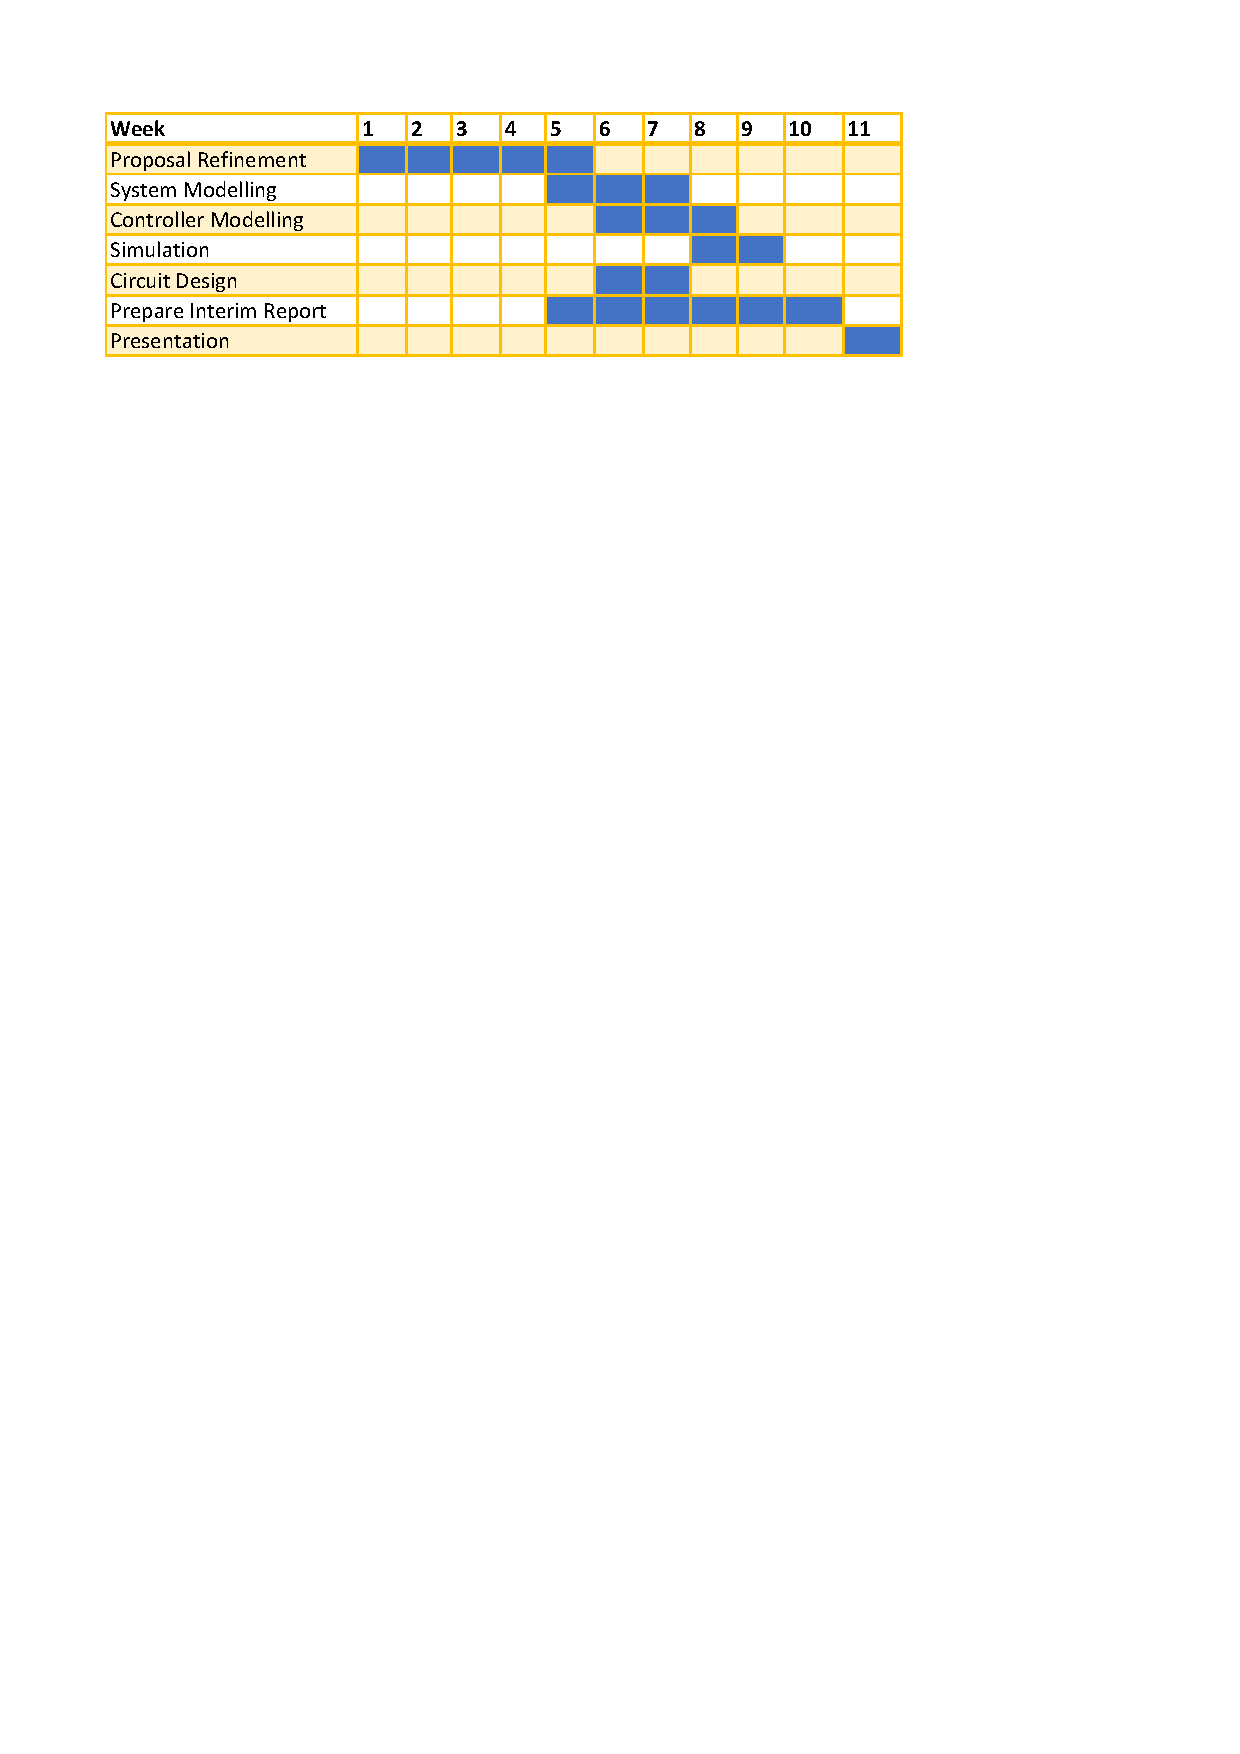
\includegraphics{Figures/workplan}
\caption{Workplan table}
\end{table}

%  \clearpage
%  \section{Appendices}
  \clearpage
%----  Bibliography  ----------------------------------------
\markright{References}                               % Erzeugt Kopfzeile
\addcontentsline{toc}{section}{References}            % Literaturverzeichnis ins Inhaltsverzeichnis
\bibliographystyle{Bib/IEEEtran}
\bibliography{Bib/References}                         % BIBTeX
\nocite{Lun01} 

                                     % Falls etwas in die Literaturliste soll, was nicht Referenziert wird
\end{document}
